%package list
\documentclass{article}
\usepackage[top=3cm, bottom=3cm, outer=3cm, inner=3cm]{geometry}
\usepackage{multicol}
\usepackage{listings}
\usepackage[utf8]{inputenc}
\usepackage{graphicx}
\usepackage{url}
%\usepackage{cite}
\usepackage{hyperref}
\usepackage{array}
%\usepackage{multicol}
\newcolumntype{x}[1]{>{\centering\arraybackslash\hspace{0pt}}p{#1}}
\usepackage{natbib} 
\usepackage{pdfpages}
\usepackage{multirow}   
\usepackage[normalem]{ulem}
\useunder{\uline}{\ul}{}
\usepackage{svg}
\usepackage{xcolor}
\usepackage{listings}
\lstdefinestyle{ascii-tree}{
    literate={├}{|}1 {─}{--}1 {└}{+}1 
  }
\lstset{basicstyle=\ttfamily,
  showstringspaces=false,
  commentstyle=\color{red},
  keywordstyle=\color{blue}
}
%\usepackage{booktabs}
\usepackage{caption}
\usepackage{subcaption}
\usepackage{float}
\usepackage{array}

\newcolumntype{M}[1]{>{\centering\arraybackslash}m{#1}}
\newcolumntype{N}{@{}m{0pt}@{}}


%%%%%%%%%%%%%%%%%%%%%%%%%%%%%%%%%%%%%%%%%%%%%%%%%%%%%%%%%%%%%%%%%%%%%%%%%%%%
%%%%%%%%%%%%%%%%%%%%%%%%%%%%%%%%%%%%%%%%%%%%%%%%%%%%%%%%%%%%%%%%%%%%%%%%%%%%
\newcommand{\itemEmail}{ shanccom@unsa.edu.pe
}
\newcommand{\itemStudent}{ Sergio Hancco Mullisaca }
\newcommand{\itemCourse}{Programacion Web 2}
\newcommand{\itemCourseCode}{}
\newcommand{\itemSemester}{II}
\newcommand{\itemUniversity}{Universidad Nacional de San Agustín de Arequipa}
\newcommand{\itemFaculty}{Facultad de Ingeniería de Producción y Servicios}
\newcommand{\itemDepartment}{Departamento Académico de Ingeniería de Sistemas e Informática}
\newcommand{\itemSchool}{Escuela Profesional de Ingeniería de Sistemas}
\newcommand{\itemAcademic}{2024 - A}
\newcommand{\itemInput}{Del 09 Mayo 2024}
\newcommand{\itemOutput}{Al 14 Junio 2024}
\newcommand{\itemPracticeNumber}{7}
\newcommand{\itemTheme}{DJANGO III}
%%%%%%%%%%%%%%%%%%%%%%%%%%%%%%%%%%%%%%%%%%%%%%%%%%%%%%%%%%%%%%%%%%%%%%%%%%%%
%%%%%%%%%%%%%%%%%%%%%%%%%%%%%%%%%%%%%%%%%%%%%%%%%%%%%%%%%%%%%%%%%%%%%%%%%%%%

\usepackage[english,spanish]{babel}
\usepackage[utf8]{inputenc}
\AtBeginDocument{\selectlanguage{spanish}}
\renewcommand{\figurename}{Figura}
\renewcommand{\refname}{Referencias}
\renewcommand{\tablename}{Tabla} %esto no funciona cuando se usa babel
\AtBeginDocument{%
	\renewcommand\tablename{Tabla}
}

\usepackage{fancyhdr}
\pagestyle{fancy}
\fancyhf{}
\setlength{\headheight}{30pt}
\renewcommand{\headrulewidth}{1pt}
\renewcommand{\footrulewidth}{1pt}
\fancyhead[L]{\raisebox{-0.2\height}{\includegraphics[width=3cm]{logo_episunsa.png}}}
\begin{figure}
    \centering
    \label{fig:enter-label}
\end{figure}
\fancyhead[C]{\fontsize{7}{7}\selectfont	\itemUniversity \\ \itemFaculty \\ \itemDepartment \\ \itemSchool \\ \textbf{\itemCourse}}
\fancyhead[R]{\raisebox{-0.2\height}{\includegraphics[width=1.2cm]{}}}
\fancyfoot[C]{\itemCourse}
\fancyfoot[R]{Página \thepage}

% para el codigo fuente
\usepackage{listings}
\usepackage{color, colortbl}
\definecolor{dkgreen}{rgb}{0,0.6,0}
\definecolor{gray}{rgb}{0.5,0.5,0.5}
\definecolor{mauve}{rgb}{0.58,0,0.82}
\definecolor{codebackground}{rgb}{0.95, 0.95, 0.92}
\definecolor{tablebackground}{rgb}{0.8, 0, 0}

\lstset{frame=tb,
	language=bash,
	aboveskip=3mm,
	belowskip=3mm,
	showstringspaces=false,
	columns=flexible,
	basicstyle={\small\ttfamily},
	numbers=none,
	numberstyle=\tiny\color{gray},
	keywordstyle=\color{blue},
	commentstyle=\color{dkgreen},
	stringstyle=\color{mauve},
	breaklines=true,
	breakatwhitespace=true,
	tabsize=3,
	backgroundcolor= \color{codebackground},
}

\begin{document}
	
	\vspace*{10px}
	
	\begin{center}	
		\fontsize{17}{17} \textbf{ Informe de Laboratorio \itemPracticeNumber}
	\end{center}
	\centerline{\textbf{\Large Tema: \itemTheme}}
	%\vspace*{0.5cm}	

	\begin{flushright}
		\begin{tabular}{|M{2.5cm}|N|}
			\hline 
			\rowcolor{tablebackground}
			\color{white} \textbf{Nota}  \\
			\hline 
			     \\[30pt]
			\hline 			
		\end{tabular}
	\end{flushright}	

	\begin{table}[H]
		\begin{tabular}{|x{4.7cm}|x{4.8cm}|x{4.8cm}|}
			\hline 
			\rowcolor{tablebackground}
			\color{white} \textbf{Estudiante} & \color{white}\textbf{Escuela}  & \color{white}\textbf{Asignatura}   \\
			\hline 
			{\itemStudent \par \itemEmail} & \itemSchool & {\itemCourse \par Semestre: \itemSemester \par Código: \itemCourseCode}     \\
			\hline 			
		\end{tabular}
	\end{table}		
	
	\begin{table}[H]
		\begin{tabular}{|x{4.7cm}|x{4.8cm}|x{4.8cm}|}
			\hline 
			\rowcolor{tablebackground}
			\color{white}\textbf{Laboratorio} & \color{white}\textbf{Tema}  & \color{white}\textbf{Duración}   \\
			\hline 
			\itemPracticeNumber  & \itemTheme & 04 horas   \\
			\hline 
		\end{tabular}
	\end{table}
	
	\begin{table}[H]
		\begin{tabular}{|x{4.7cm}|x{4.8cm}|x{4.8cm}|}
			\hline 
			\rowcolor{tablebackground}
			\color{white}\textbf{Semestre académico} & \color{white}\textbf{Fecha de inicio}  & \color{white}\textbf{Fecha de entrega}   \\
			\hline 
			\itemAcademic & \itemInput &  \itemOutput  \\
			\hline 
		\end{tabular}
	\end{table}
	
	\section{Tarea}
	\begin{itemize}		
		\item Informe de laboratorio
            \item Video en Flip
		\item Ejercicios Propuestos
        
	\end{itemize}
		
	\section{Equipos, materiales y temas utilizados}
	\begin{itemize}
		\item VS
		\item Git 2.39.2.
		\item Cuenta en GitHub con el correo institucional.
	\end{itemize}
    \clearpage
    
	\section{URL de Repositorio Github}
	\begin{itemize}
        \item URL del video en yt.
		\item \url{https://youtu.be/dkZBugjlI2s}
        \item URL del video en flip.
		\item \url{https://flip.com/s/kj5APzDKgEHZ}
        \item URL del GITHUB.
            \item \url{https://github.com/shanccom/Programacion_Web_2.git}
	\end{itemize}
	
	\section{Actividades}
	\subsection{EJERCICIOS PROPUESTOS}
        \item VIDEOS (1-4): CREACION DE CLASES EN MODELS

        \begin{lstlisting}[language=Python, caption=models.py]
from django.db import models

# Create your models here.

class Languaje(models.Model):
    name = models.CharField(max_length = 10)

    def __str__(self):
        return self.name
        
class FrameWork(models.Model):
    name = models.CharField(max_length = 10)
    languaje = models.ForeignKey(Languaje, on_delete = models.CASCADE)

    def __str__(self):
        return self.name
    
class Movie(models.Model):
    name = models.CharField(max_length = 10)

    def __str__(self):
        return self.name
    
class Character(models.Model):
    name = models.CharField(max_length = 10)
    movies = models.ManyToManyField(Movie)

    def __str__(self):
        return self.name

        \end{lstlisting}
        \item Evidencia de la generacion de framework
        \newline\newline \newline\newline \newline\newline 
        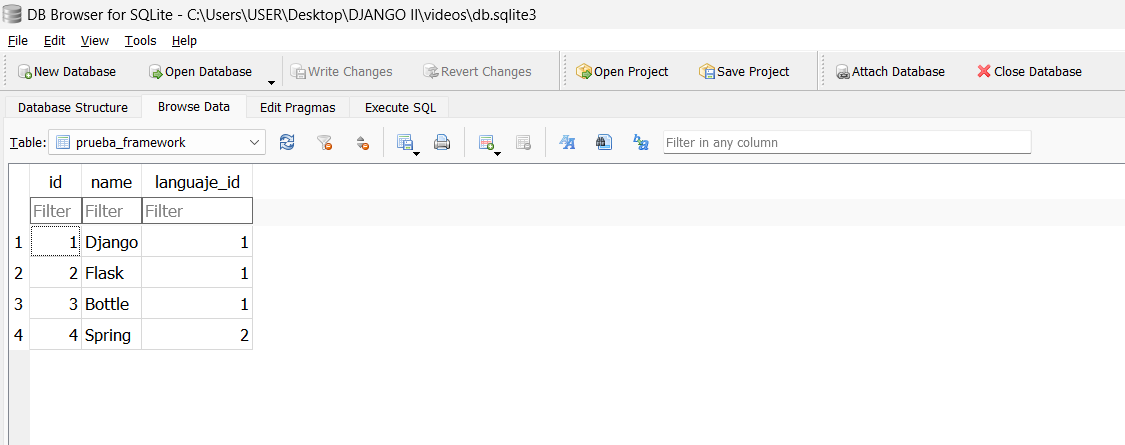
\includegraphics[width=1\textwidth,keepaspectratio]{IMAGENES/Evidencia Primer video I.png}
        \newline \newline\newline 
        \item Uso de Shell para la creacion
        \newline \newline\newline  
        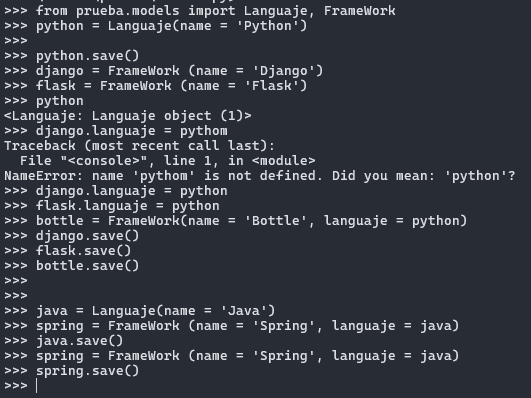
\includegraphics[width=1\textwidth,keepaspectratio]{IMAGENES/Evidencia Primer video IIi.png}
        \newline\newline \newline\newline 
        \item Uso de Shell (COMANDOS)
        \newline \newline\newline
        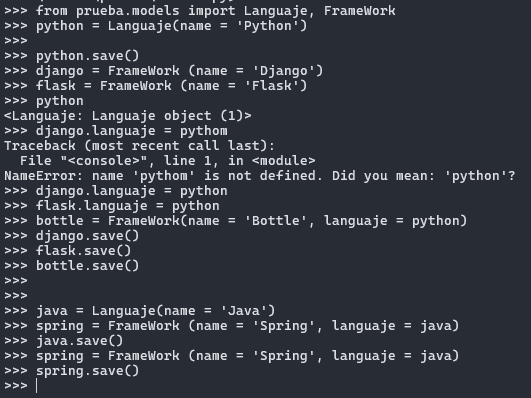
\includegraphics[width=1\textwidth,keepaspectratio]{IMAGENES/Evidencia Primer video IIi.png}
        \newline
        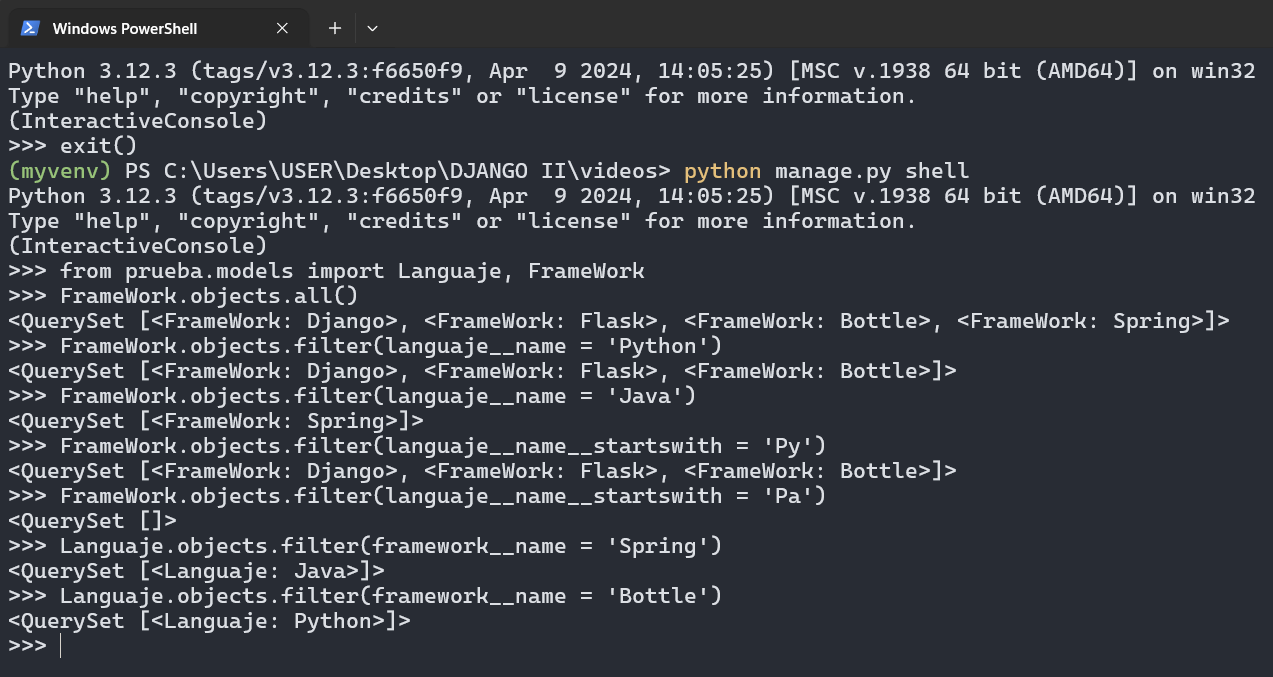
\includegraphics[width=1\textwidth,keepaspectratio]{IMAGENES/Evidencia Segundo Video I.png}
        \newline
        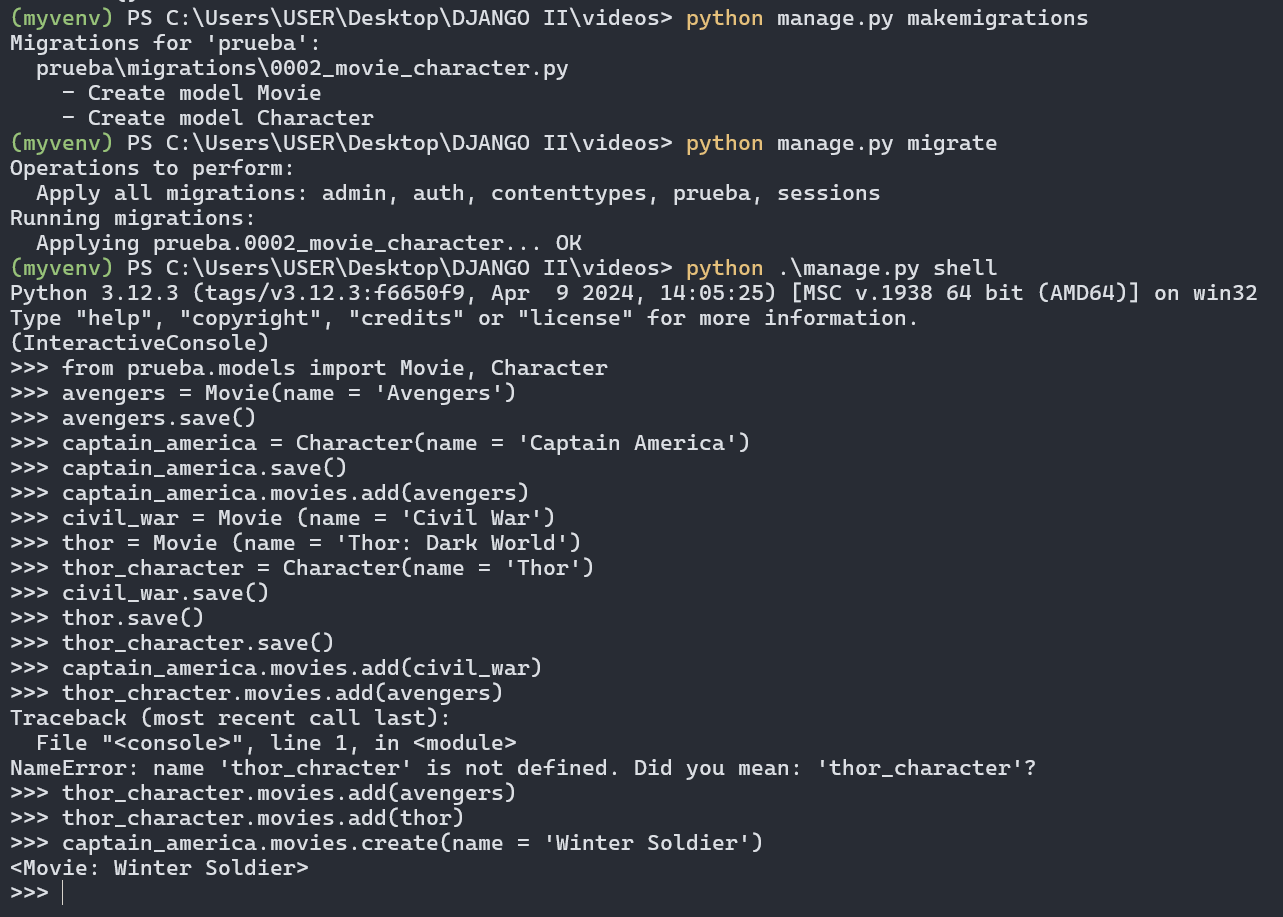
\includegraphics[width=1\textwidth,keepaspectratio]{IMAGENES/Evidencia Tercer video I.png}
        \newline \newline \newline\newline \newline
        \item Muestra de la relacion character movies
        \newline \newline\newline
        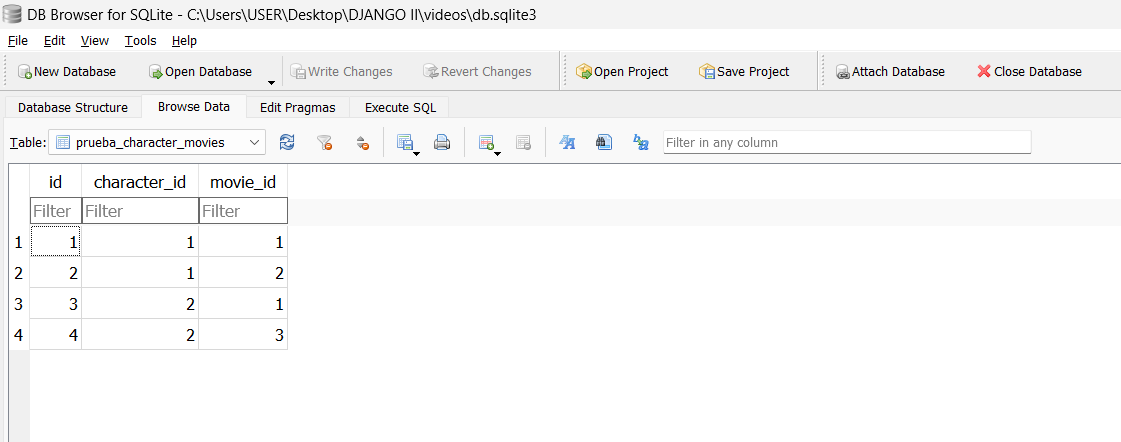
\includegraphics[width=1\textwidth,keepaspectratio]{IMAGENES/Evidencia Tercer video II.png}
        \newline \
        \item Muestra character
        \newline \newline
        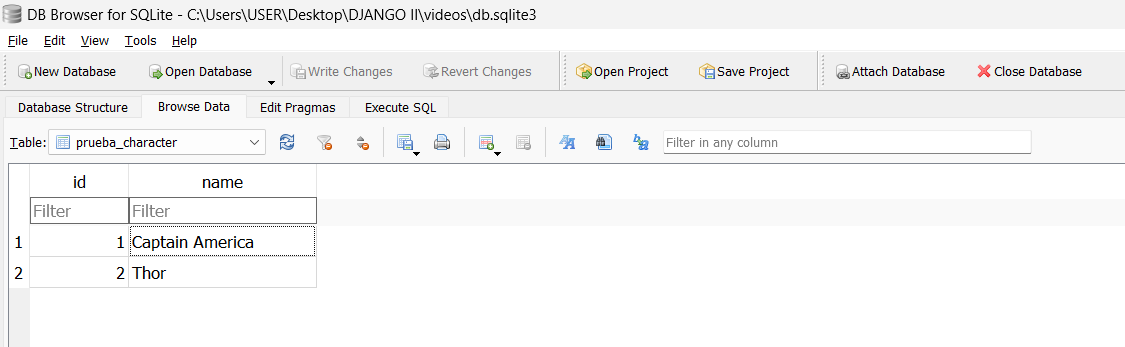
\includegraphics[width=1\textwidth,keepaspectratio]{IMAGENES/Evidencia Tercer video III.png}
        \newline \newline 
        \item Muestra movie
        \newline \newline
        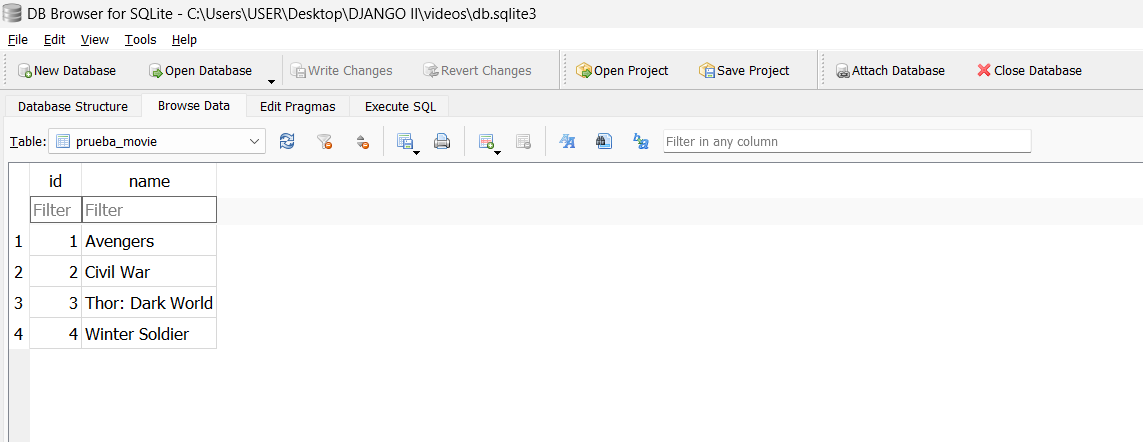
\includegraphics[width=1\textwidth,keepaspectratio]{IMAGENES/Evidencia Tercer video IV.png}
        \newline \newline 
        \item Metodo para que devuelva todas las peliculas
        \newline \newline\newline
        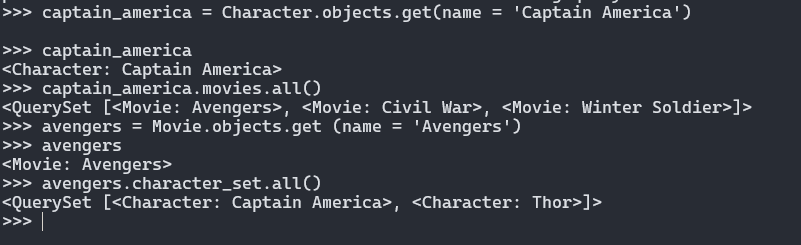
\includegraphics[width=1\textwidth,keepaspectratio]{IMAGENES/Evidencia Cuarto video I.png}
        \newline

        \item VIDEOS 5: HTML A PDF
        \item Metodos n views
        \begin{lstlisting}[language=Python, caption=views.py]
import locale

from . import renderers


def invoice_view(request):
    context = {
        "bill_to": "Danilo",
        "invoice_number": "007cae",
        "amount": 100_000,
        "date": "2024-06-14",
    }
    return renderers.render_to_pdf("pdfs/invoice.html", context)


def advanced_pdf_view(request):
    locale.setlocale(locale.LC_ALL, "")
    invoice_number = "007cae"
    context = {
        "bill_to": "Sergio",
        "invoice_number": f"{invoice_number}",
        "amount": locale.currency(100_000, grouping=True),
        "date": "2024-23-10",
        "pdf_title": f"Invoice #{invoice_number}",
    }
    response = renderers.render_to_pdf("pdfs/invoice.html", context)
    if response.status_code == 404:
        raise HTTP404("Invoice not found")

    filename = f"Invoice_{invoice_number}.pdf"
    """
    Tell browser to view inline (default)
    """
    content = f"inline; filename={filename}"
    download = request.GET.get("download")
    if download:
        """
        Tells browser to initiate download
        """
        content = f"attachment; filename={filename}"
    response["Content-Disposition"] = content
    return response
    return response
        \end{lstlisting}  

        \item CAPTURAS DE EVIDENCIA
        \item USO BASICO
        \newline \newline\newline\newline 
        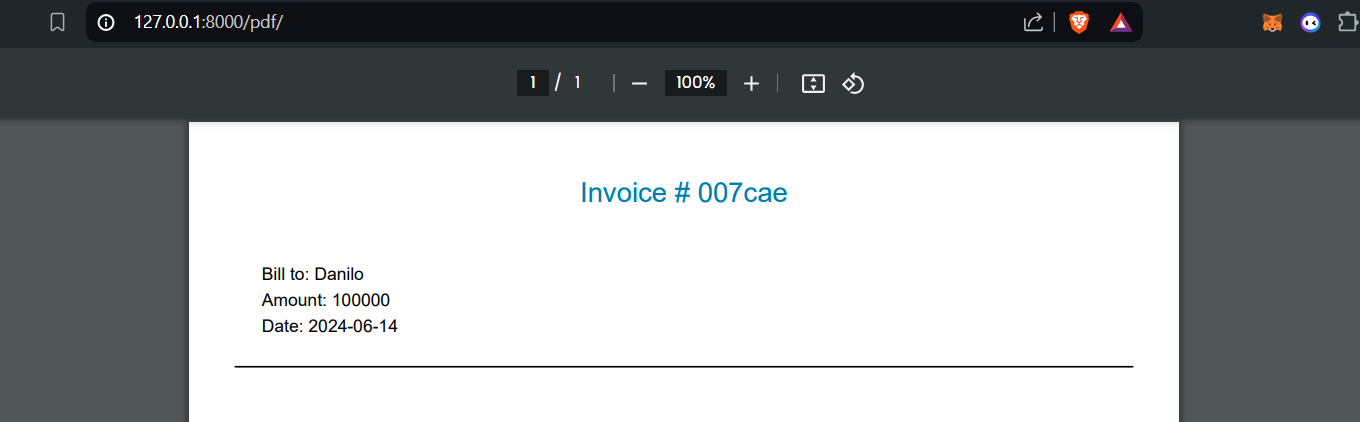
\includegraphics[width=1\textwidth,keepaspectratio]{IMAGENES/Evidencia Quinto video I.png}
        \newline \newline\newline
        \item USO AVANZADO
        \newline \newline\newline\newline 
        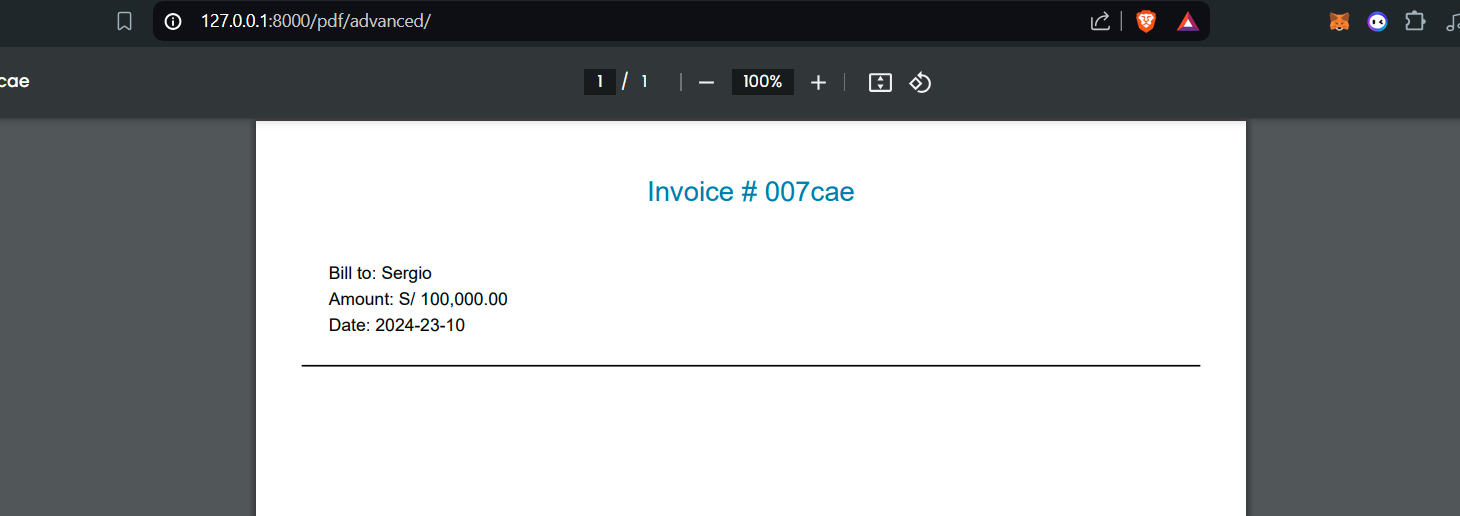
\includegraphics[width=1\textwidth,keepaspectratio]{IMAGENES/Evidencia Quinto video II.png}
        \newline \newline\newline

        \item VIDEOS 6: ENVIO DE GMAIL
        \begin{lstlisting}[language=Python, caption=views.py]
from django.shortcuts import render
from django.core.mail import send_mail

def index(request):

    send_mail('Hola',
    'Mensaje automatico PRUEBA 1', 
    'correo@gmail.com',
    ['correo@gmail.com'],
    fail_silently = False)

    return render(request, 'send/index.html')

        \end{lstlisting}  
        \begin{lstlisting}[language=Python, caption=settings.py]

EMAIL_BACKEND = 'django.core.mail.backends.smtp.EmailBackend'
EMAIL_HOST = 'smtp.gmail.com'
EMAIL_PORT = 587
EMAIL_HOST_USER = 'correo@gmail.com'
EMAIL_USE_TLS = True    

        \end{lstlisting}  

        \item EVIDENCIA DEL ENVIO
        \newline \newline\newline\newline 
        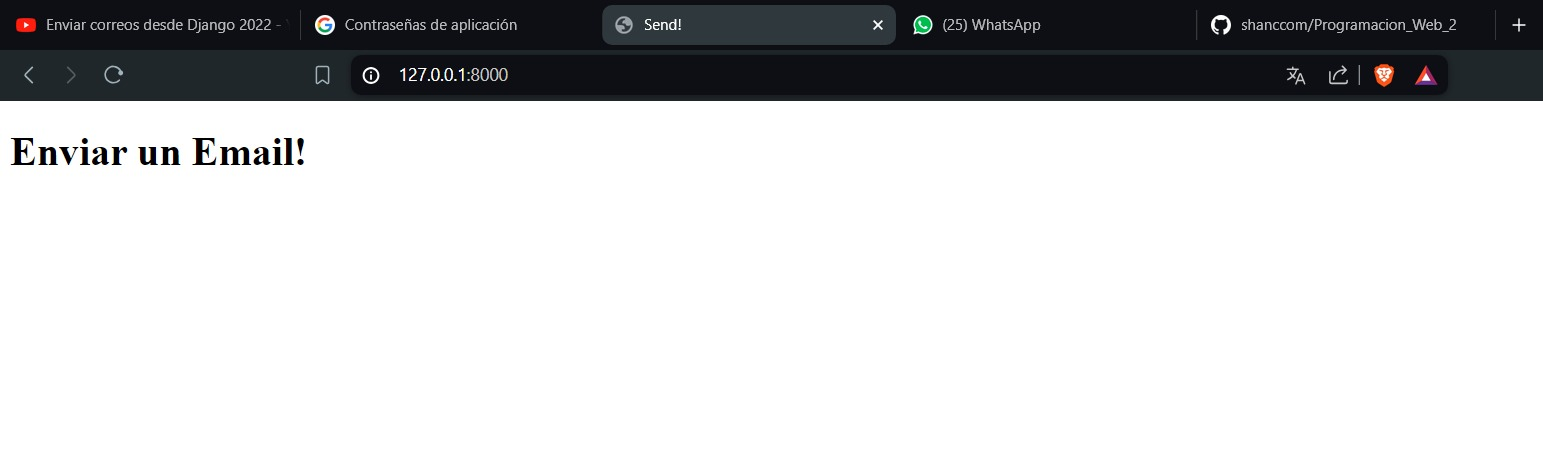
\includegraphics[width=0.6\textwidth,keepaspectratio]{Evidencia Sexto video I.png}
        \newline 
        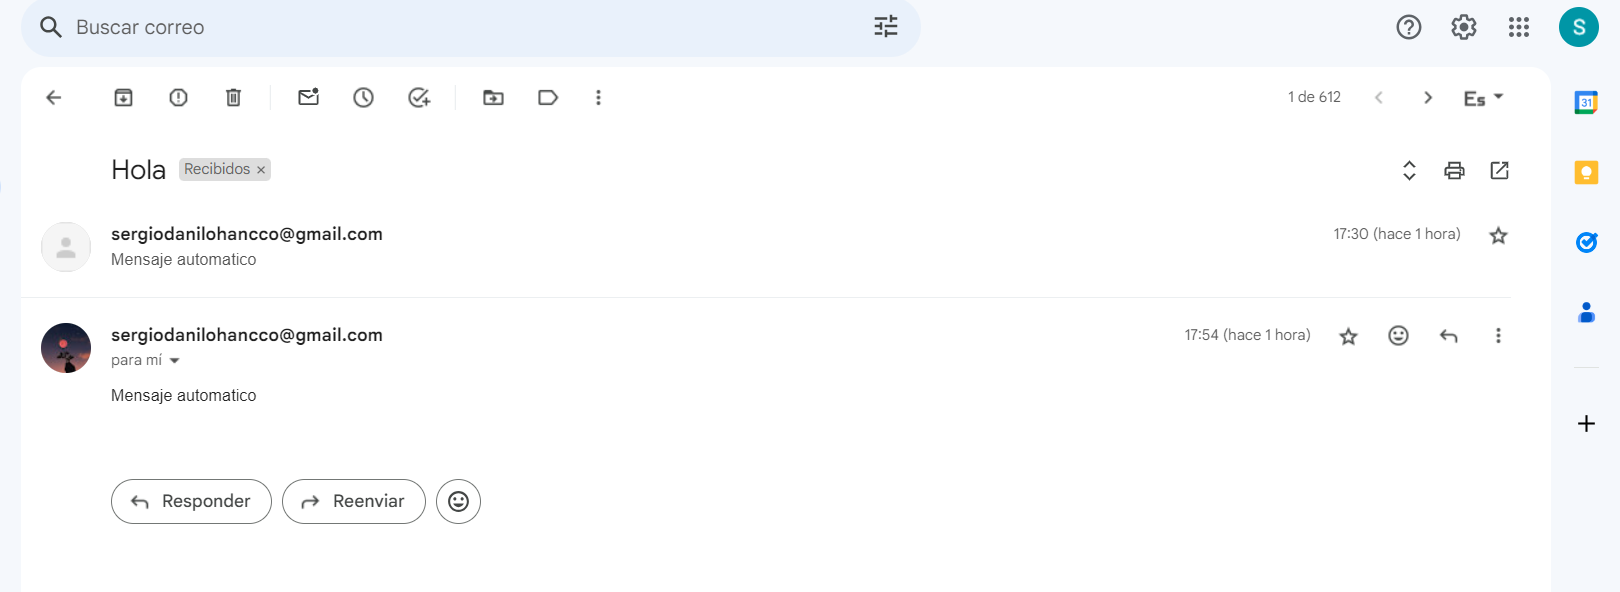
\includegraphics[width=1\textwidth,keepaspectratio]{Evidencia Sexto video II.png}

    \clearpage

	\section{\textcolor{red}{Rúbricas}}
	
	\subsection{\textcolor{red}{Entregable Informe}}
	\begin{table}[H]
		\caption{Tipo de Informe}
		\setlength{\tabcolsep}{0.5em} % for the horizontal padding
		{\renewcommand{\arraystretch}{1.5}% for the vertical padding
		\begin{tabular}{|p{3cm}|p{12cm}|}
			\hline
			\multicolumn{2}{|c|}{\textbf{\textcolor{red}{Informe}}}  \\
			\hline 
			\textbf{\textcolor{red}{Latex}} & \textcolor{blue}{El informe está en formato PDF desde Latex,  con un formato limpio (buena presentación) y facil de leer.}   \\ 
			\hline 
			
			
		\end{tabular}
	}
	\end{table}
	

	
	\subsection{\textcolor{red}{Rúbrica para el contenido del Informe y demostración}}
	\begin{itemize}			
		\item El alumno debe marcar o dejar en blanco en celdas de la columna \textbf{Checklist} si cumplio con el ítem correspondiente.
		\item Si un alumno supera la fecha de entrega,  su calificación será sobre la nota mínima aprobada, siempre y cuando cumpla con todos lo items.
		\item El alumno debe autocalificarse en la columna \textbf{Estudiante} de acuerdo a la siguiente tabla:
	
		\begin{table}[ht]
			\caption{Niveles de desempeño}
			\begin{center}
			\begin{tabular}{ccccc}
    			\hline
    			 & \multicolumn{4}{c}{Nivel}\\
    			\cline{1-5}
    			\textbf{Puntos} & Insatisfactorio 25\%& En Proceso 50\% & Satisfactorio 75\% & Sobresaliente 100\%\\
    			\textbf{2.0}&0.5&1.0&1.5&2.0\\
    			\textbf{4.0}&1.0&2.0&3.0&4.0\\
    		\hline
			\end{tabular}
		\end{center}
	\end{table}	
	
	\end{itemize}
	
	\begin{table}[H]
		\caption{Rúbrica para contenido del Informe y demostración}
		\setlength{\tabcolsep}{0.5em} % for the horizontal padding
		{\renewcommand{\arraystretch}{1.5}% for the vertical padding
		%\begin{center}
		\begin{tabular}{|p{2.7cm}|p{7cm}|x{1.3cm}|p{1.2cm}|p{1.5cm}|p{1.1cm}|}
			\hline
    		\multicolumn{2}{|c|}{Contenido y demostración} & Puntos & Checklist & Estudiante & Profesor\\
			\hline
			\textbf{1. GitHub} & Hay enlace URL activo del directorio para el  laboratorio hacia su repositorio GitHub con código fuente terminado y fácil de revisar. &2 &X &2 & \\ 
			\hline
			\textbf{2. Commits} &  Hay capturas de pantalla de los commits más importantes con sus explicaciones detalladas. (El profesor puede preguntar para refrendar calificación). &4 &X &4 &  \\ 
			\hline 
			\textbf{3. Código fuente} &  Hay porciones de código fuente importantes con numeración y explicaciones detalladas de sus funciones. &2 &X &2 & \\ 
			\hline 
			\textbf{4. Ejecución} & Se incluyen ejecuciones/pruebas del código fuente  explicadas gradualmente. &2 &X &1 & \\ 
			\hline			
			\textbf{5. Pregunta} & Se responde con completitud a la pregunta formulada en la tarea.  (El profesor puede preguntar para refrendar calificación).  &2 &X &2 & \\ 
			\hline	
			\textbf{6. Fechas} & Las fechas de modificación del código fuente estan dentro de los plazos de fecha de entrega establecidos. &2 &X &2 & \\ 
			\hline 
			\textbf{7. Ortografía} & El documento no muestra errores ortográficos. &2 &X &2 & \\ 
			\hline 
			\textbf{8. Madurez} & El Informe muestra de manera general una evolución de la madurez del código fuente,  explicaciones puntuales pero precisas y un acabado impecable.   (El profesor puede preguntar para refrendar calificación).  &4 &X &4 & \\ 
			\hline
			\multicolumn{2}{|c|}{\textbf{Total}} &20 & &19 & \\ 
			\hline
		\end{tabular}
		%\end{center}
		%\label{tab:multicol}
		}
	\end{table}
	
\clearpage
	   
	
%\clearpage
%\bibliographystyle{apalike}
%\bibliographystyle{IEEEtranN}
%\bibliography{bibliography}
			
\end{document}